\chapter{\selectlanguage{greek}Θεωρητικό υπόβαθρο}

Στο κεφάλαιο αυτό παρουσιάζονται αναλυτικά οι τεχνολογίες που είναι απαραίτητες για την κατανόηση της διπλωματικής εργασίας.

\section{\selectlanguage{greek}\en{Deep Learning}\cite{LeCun2015}}

Η υπολογιστική εκμάθηση \en{(Machine Learning)} είναι η κινητήριος δύναμη για διάφορες εκφάνσεις της σύγχρονης κοινωνίας: από αναζητήσεις στο διαδίκτυο μέχρι και φιλτράρισμα περιεχομένου σε κοινωνικά δίκτυα και προτάσεις αγορών σε ηλεκτρονικά καταστήματα. 
Ολοένα συχνότερη και συνηθέστερη γίνεται η εμφάνιση του σε προϊόντα ευρείας κατανάλωσης όπως κάμερες και κινητά τηλέφωνα. 
Τα συστήματα υπολογιστικής εκμάθησης χρησιμοποιούνται για την αναγνώριση αντικειμένων σε εικόνες, την αυτόματη καταγραφή προφορικού λόγου, την αντιστοίχηση προϊόντων - νέων - δημοσιεύσεων με τις προτιμήσεις χρηστών. 
Σε όλες αυτές τις εφαρμογές, είναι αυξανόμενη η χρήση ενός σετ τεχνικών που φέρει το όνομα \en{Deep Learning}.

Οι συμβατικές τεχνικές υπολογιστικής εκμάθησης είχαν περιορισμένη δυνατότητα χρήσης της ανεπεξέργαστης πληροφορίας. 
Για δεκαετίες, η σχεδίαση και η υλοποίηση ενός συστήματος αναγνώρισης προτύπων ή υπολογιστικής εκμάθησης, απαιτούσε προσεκτική προσέγγιση και σημαντική εξειδίκευση στον εκάστοτε τομέα. 
Αυτό επειδή χρειαζόταν η μετατροπή της ανεπεξέργαστης πληροφορίας σε μία κατάλληλη εσωτερική αναπαράσταση, την οποία το υποσύστημα εκμάθησης -- συχνότερα ένας ταξινομητής -- θα χρησιμοποιούσε για αναγνωρίσει πρότυπα στις διάφορες εισόδους.

Η εκμάθηση αναπαραστάσεων είναι ένα σύνολο μεθόδων που επιτρέπουν σε ένα σύστημα να ανακαλύψει αυτόματα ποιες ακριβώς αναπαραστάσεις της ανεπεξέργαστης πληροφορίας χρειάζεται, για να επιτελέσει την αναγνώριση προτύπων ή την ταξινόμηση. 
Οι μέθοδοι \en{Deep Learning} είναι μέθοδοι εκμάθησης αναπαραστάσεων με πολλαπλά επίπεδα αναπαράστασης, που αποτελούνται από την σύνθεση απλών, μη γραμμικών υποσυστημάτων, το καθένα από τα οποία -- ξεκινώντας από την ανεπεξέργαστη είσοδο -- μετατρέπει την αναπαράσταση της πληροφορίας σε μια λίγο πιο υψηλά αφαιρετική μορφή σε κάθε επίπεδο.
Με την χρήση αρκετών τέτοιων μετατροπών το σύστημα μπορεί να μάθει εξαιρετικά σύνθετες λειτουργίες.
Για διαδικασίες ταξινόμησης, τα υψηλότερα επίπεδα αναπαράστασης ενισχύουν πτυχές τις εισόδου που είναι πιο σημαντικές για τον τελικό σκοπό.
Σε μία εικόνα, για παράδειγμα, η οποία αναπαριστάται ως διάνυσμα τιμών εικονοκυττάρων, τα χαρακτηριστικά που μαθαίνονται στο πρώτο επίπεδο είναι συνήθως πληροφορία για την παρουσία ή την απουσία ακμών σε συγκεκριμένες θέσεις και προσανατολισμούς.
Στο δεύτερο επίπεδο, συνήθως εντοπίζονται μοτίβα μέσω των διαφόρων διατάξεων των ακμών, χωρίς να χρειάζεται τα μοτίβα να επαναλαμβάνονται επακριβώς.
Στο τρίτο επίπεδο μπορούν να αναγνωριστούν σύνολα μοτίβων σε μεγάλους συνδυασμούς που αντιστοιχούν σε γνωστά αντικείμενα ή μέρη τους.
Τα επόμενα επίπεδα, παρόμοια, εντοπίζουν πιο σύνθετα αντικείμενα ως συνδυασμούς απλούστερων μερών.
Το βασικότερο στοιχείο του \en{Deep Learning} είναι πως τα επίπεδα που εντοπίζουν χαρακτηριστικά και δομές δεν είναι σχεδιασμένα από τους ανθρώπους: μαθαίνονται από τα δεδομένα χρησιμοποιώντας γενικευμένες διαδικασίες εκμάθησης.

Η χρήση του \en{Deep Learning} έχει βοηθήσει στην αντιμετώπιση προβλημάτων που δυσκόλευαν την κοινότητα της τεχνητής νοημοσύνης εδώ και χρόνια. 
Αποδεικνύεται να έχει επιδόσεις χωρίς προηγούμενο στον εντοπισμό πολύπλοκων δομών σε δεδομένα πολλών διαστάσεων και για αυτό είναι εφαρμόσιμο σε πολλούς διαφορετικούς τομείς, επιστημονικούς, επιχειρησιακούς και κοινωνικοπολιτικούς.
Πέρα από επαναστατικές επιδόσεις στην αναγνώριση φωνής και εικόνας, έχει ξεπεράσει άλλες τεχνικές υπολογιστικής εκμάθησης στην πρόβλεψη συμπεριφοράς μορίων φαρμάκων, στην ανάλυση δεδομένων από επιταχυντές σωματιδίων, στην ανακατασκευή εγκεφαλικών κυκλωμάτων και στην πρόβλεψη των επιπτώσεων μεταλλάξεων μη κωδικοποιητικού \en{DNA} στις γονιδιακές εκφράσεις και ασθένειες.
Ίσως, οι πιο αναπάντεχα υποσχόμενες επιδόσεις έγιναν στον κλάδο της επεξεργασίας φυσικής γλώσσας, συγκεκριμένα στην εντοπισμό θεμάτων, την ανάλυση συναισθήματος, τις ερωτήσεις - απαντήσεις και την μετάφραση.
%TODO References for best results from paper Deep Learning Hinton Bengio lecun

\section{\selectlanguage{greek}\en{Supervised Learning}\cite{LeCun2015}}

Η πιο συνήθης μορφή υπολογιστικής εκμάθησης, είτε \en{Deep Learning} είτε όχι, είναι αυτή της επιτηρούμενης εκμάθησης.
Ας θεωρήσουμε πως θέλουμε να φτιάξουμε ένα σύστημα που αποφασίζει τι περιέχει μια εικόνα, όπως ένα σπίτι, ένα αυτοκίνητο, έναν άνθρωπο ή μία γάτα.
Αρχικά, συλλέγουμε ένα αρκετά μεγάλο σύνολο δεδομένων με εικόνες στα οποία σημειώνεται τι αντικείμενο από τα παραπάνω περιέχει κάθε εικόνα.
Κατά τη διάρκεια της εκπαίδευσης, δείχνουμε στο σύστημα μια εικόνα και αυτό παράγει μία πρόβλεψη, στη μορφή ενός διανύσματος με σκορ για κάθε κατηγορία.
Θέλουμε η επιθυμητή κατηγορία να έχει το μεγαλύτερο σκορ πρόβλεψης, αλλά αυτό είναι πολύ δύσκολο πριν την εκπαίδευση.
Υπολογίζουμε μία συνάρτηση στόχου με την οποία μετράμε το λάθος (ή την απόσταση) μεταξύ των αποτελεσμάτων του συστήματος και τον επιθυμητών αποτελεσμάτων.
Το σύστημα, ύστερα, προσαρμόζει τις εσωτερικές του παραμέτρους ώστε να μειώσει το λάθος.
Οι εσωτερικές παράμετροι, που συχνότερα στη βιβλιογραφία απαντώνται ως βάρη, είναι πραγματικοί αριθμοί που ορίζουν την λειτουργικότητα εισόδου-εξόδου του συστήματος.
Σε ένα τυπικό \en{Deep Learning} σύστημα, οι εσωτερικές παράμετροι και τα παραδείγματα που χρησιμοποιούμε για την εκμάθηση του συστήματος μπορεί να είναι εκατοντάδες εκατομμύρια σε αριθμό. 

Για την κατάλληλη προσαρμογή των βαρών, ο αλγόριθμος εκμάθησης υπολογίζει ένα διάνυσμα κλίσης, για κάθε βάρος, που δείχνει κατά πόσο και προς ποια κατεύθυνση αλλάζει το λάθος αν αλλάξουμε απειροστά το αντίστοιχο βάρος.
Το διάνυσμα των βαρών τελικά ρυθμίζεται έτσι ώστε να έχει αντίθετη φορά με το διάνυσμα κλίσης.
Η διαδικασία αυτή είναι μία προσπάθεια ελαχιστοποίησης της συνάρτησης λάθους και μεταγενέστερα της μείωσης, κατά μέσο όρο, των λαθών προβλέψεων του συστήματος.

\begin{figure}[tph]
	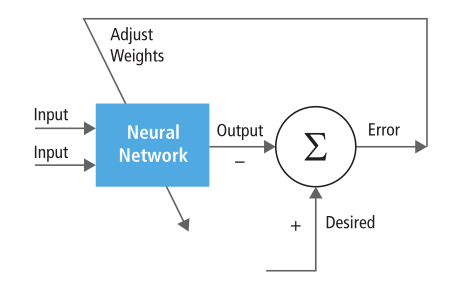
\includegraphics[width=0.8\textwidth, keepaspectratio]{images/training.png}
	\centering 
	\caption{Ένα τυπικό δομικό διάγραμμα επιτηρούμενης εκμάθησης.}
	\label{fig:training}
\end{figure}

Στην πλειοψηφία της σύγχρονης βιβλιογραφίας, και στην παρούσα διπλωματική, ο αλγόριθμος ελαχιστοποίησης που χρησιμοποιείται είναι ο \en{stochastic gradient descent (SGD)}.
Αυτός συνίσταται από την επίδειξη λίγων κάθε φορά, σωστά επισημασμένων, παραδειγμάτων στο σύστημα, τον υπολογισμό των προβλέψεων και του λάθους, τον υπολογισμό του διανύσματος κλίσης και την ρύθμιση των βαρών.
Η παραπάνω διαδικασία επαναλαμβάνεται για πολλά μικρά σετ παραδειγμάτων, μέχρι η συνάρτηση στόχου να σταματήσει να μειώνεται.
Μετά την εκπαίδευση, οι επιδόσεις του συστήματος μετρώνται σε ένα σύνολο διαφορετικών παραδειγμάτων, έτσι ώστε να εξεταστεί η ικανότητα γενίκευσης του συστήματος σε εισόδους που βλέπει για πρώτη φορά.
 %TODO What is an objective function, στοχος
 
\section{\selectlanguage{greek}\en{Recurrent Neural Networks}}

Τα αναδραστικά νευρωνικά δίκτυα (\en{Recurrent Neural Networks - RNNs}) είναι μία προσαρμογή των κλασσικών, πλήρως συνδεδεμένων νευρωνικών δικτύων, έτσι ώστε τα πρώτα να μπορούν να διαχειριστούν ακολουθίες. 
Σε κάθε χρονική στιγμή, τα \en{RNNs} δέχονται μια είσοδο, ενημερώνουν την εσωτερική τους κατάσταση και παράγουν μία έξοδο.
Η πολυδιάστατη εσωτερική κατάσταση, που συχνά απαντάται στη βιβλιογραφία ως κρυφή κατάσταση (\en{hidden state}), και η μη γραμμική εξέλιξη της διαχειριζόμενης πληροφορίας δίνουν στα αναδραστικά νευρωνικά δίκτυα μεγάλη εκφραστική ευελιξία και δυνατότητα ενσωμάτωσης και διατήρησης της πληροφορίας σε μεγάλα χρονικά διαστήματα.
Ακόμα και όταν η μη γραμμική συνάρτηση που χρησιμοποιείται από κάθε στοιχείο του \en{RNN} είναι εξαιρετικά απλή, η χρήση της σε πολλά επίπεδα και η επανάληψη της σε κάθε χρονική στιγμή οδηγεί σε ένα εξαιρετικά δυναμικό σύστημα. 

Τα αναδραστικά νευρωνικά δίκτυα ορίζονται ως εξής: δεδομένης μιας ακολουθίας διανυσμάτων εισόδου $(x_1, x_2, ..., x_T)$, το σύστημα υπολογίζει μία ακολουθία κρυφών κατάστασεων $(h_1, h_2, ..., h_T)$ και μία παράγει μια ακολουθία εξόδων $(ο_1, ο_2, ..., ο_T)$, σύμφωνα με τον κάτωθι αλγόριθμο:

\selectlanguage{english}

\begin{algorithm}
\caption{\en{RNN}}
\begin{algorithmic}
\FOR { $t = 1$ to $T$}
\STATE \begin{equation}
h_t = \tanh(W_h x_t + W_{hh} h_{t-1} + b_h)\label{eq:h}
\end{equation}
\STATE \begin{equation}
o_t = W_{oh} h_t + b_o
\end{equation}
\ENDFOR
\end{algorithmic}
\end{algorithm}
\selectlanguage{greek}

Σε αυτές τις εξισώσεις, το $W_{hx}$ είναι ο πίνακας βαρών από την είσοδο στην κρυφή κατάσταση, το $W_{hh}$ είναι ο πίνακας απο την κρυφή κατάσταση στην κρυφή κατάσταση, το $W_{oh}$ είναι ο πίνακας βαρών από την κρυφή κατάσταση στην έξοδο και τα $b_h, b_o$ είναι οι σταθεροί όροι.
Η μη ορισμένη σχέση $W_{hh}h_{t-1}$ στη χρονική στιγμή $t = 1$ αντικαθίσταται με ένα διάνυσμα αρχικοποίησης, $h_{init}$, και η συνάρτηση της υπερβολικής εφαπτομένης, $\tanh$, εφαρμόζεται κατά στοιχείο.

\begin{figure}[tph]
	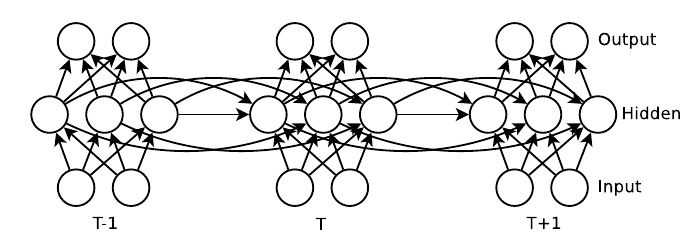
\includegraphics[width=\textwidth, keepaspectratio]{images/rnn.png}
	\centering 
	\caption{To αναδραστικό νευρωνικό δίκτυο <<\tg{ανοιγμένο}>> στον χρόνο}
	\label{fig:rnn}
\end{figure}

Οι παράγωγοι των στοιχειδών μερών του δικτύου είναι εύκολο να υπολογιστούν, με τη μέθοδο της προς τα πίσω διάδοσης σφάλματος, \cite{Graves2013}, οπότε ίσως η εκπαίδευση ενός τέτοιου συστήματος φαίνεται εύκολη.
Στην πραγματικότητα, η σχέση μεταξύ των παραμέτρων του \en{RNN} και της δυναμικής του είναι εξαιρετικά ασταθής, γεγονός που καθιστά τον αλγόριθμο \en{SGD} αναποτελεσματικό.
Αυτό τεκμηριώνεται απο τους \en{Pascanu et al.} \cite{Pascanu2012} που αποδεικνύουν πως τα διανύσματα κλίσεων τείνουν να μηδενίζονται (ή σπανιότερα να απειρίζονται) εκθετικά με την διάδοση του σφάλματος στο χρόνο.
Στη σχετική βιβλιογραφία αυτό απαντάται ως πρόβλημα εξαφάνισης ή έκρηξης των διανυσμάτων κλίσης (<<\en{vanishing or exploding gradients problem}>>)
Το παραπάνω χρησιμοποιήθηκε ως επιχείρημα για το ότι τα αναδραστικά νευρωνικά δίκτυα δεν μπορούν να αποτυπώσουν εξαρτήσεις με μεγάλη χρονική απόσταση μεταξύ τους, οταν ο χρησιμοποιείται ο αλγόριθμος \en{SGD}.
Επιπρόσθετα, ο περιστασιακός απειρισμός των διανυσμάτων κλίσης αυξάνει τη διακύμανση τους και κάνει την εκμάθηση ασταθή.
Τα θεωρητικά αποτελέσματα αυτά, δεδομένου πως ο \en{SGD} ήταν ο βασικότερος αλγόριθμος εκπαίδευσης νευρωνικών δικτύων, σε συνδυασμό με την εμπειρική δυσκολία εκπαίδευσης των \en{RNNs} οδήγησε στη σχεδόν ολοκληρωτική εγκατάλειψη της σχετικής έρευνας.

\section{\selectlanguage{greek}Εκπαίδευση των \en{Recurrent Neural Networks}}
\subsection{\en{Long Short-Term Memory Units}\cite{Hochreiter1997}}

Ένας τρόπος να αντιμετωπιστεί η αδυναμία που παρουσιάζουν τα \en{RNNs} στην εκμάθησης δομών με μακρινές, στο χρόνο, αλληλεξαρτήσεις είναι η τροποποίηση του μοντέλου ώστε να έχει στοιχεία με μνήμη.
Η προσέγγιση αυτή ονομάζεται \en{Long Short-Term Memory} και γνωρίζει ευρεία χρήση. Οι σχέσεις που ορίζουν κάθε στοιχείο μνήμης είναι:

\begin{equation}
i_t = \sigma{(W_{xi}x_t + W_{hi}h_{t-1} + W_{ci}c_{t-1} + b_i)}
\end{equation}
\begin{equation}
f_t = \sigma{(W_{xf}x_t + W_{hf}h_{t-1} + W_{cf}c_{t-1} + b_f)}
\end{equation}
\begin{equation}
c_t = f_t c_{t-1} + i_t \tanh{(W_{xc} h_{t-1} + W_{cf} c_{t-1} + b_c)}\label{eq:c}
\end{equation}
\begin{equation}
o_t = \sigma(W_{xo}x_t + W_{ho} h_{t-1} + W_{co} c_t + b_o)
\end{equation}
\begin{equation}
h_t = o_t\tanh{c_t}
\end{equation}

Το $\sigma$ είναι η σιγμοειδής συνάρτηση, $i, f, o$ και $c$ είναι αντίστοιχα η πύλη εισόδου, η πύλη απώλειας μνήμης, η πύλη εξόδου και η μνήμη.
Τα τελευταία είναι διανύσματα με διαστάσεις ίδιες με του διανύσματος $h$ (βλ. εξίσωση \ref{eq:h}, που ταυτίζεται με τον δεύτερο όρο της εξίσωσης \ref{eq:c}).
Οι δείκτες των πινάκων βαρών $W$ έχουν το προφανές νόημα, για παράδειγμα ο $W_{hi}$ είναι ο πίνακας βαρών  κρυφής κατάστασης -- εισόδου, ο $W_{xo}$ είναι πίνακας βαρών εισόδου -- εξόδου κ.ο.κ. Οι πίνακες βαρών από την μνήμη στις πύλες είναι διαγώνιοι, έτσι το στοιχείο $m$ σε κάθε πύλη δέχεται είσοδο μόνο από το στοιχείο $m$ του διανύσματος μνήμης.

Μια πιο διαισθητική εξήγηση του συστήματος \en{LSTM} είναι η εξής:
Η μνήμη $c$, σε κάθε επανάληψη της λειτουργίας του αναδραστικού νευρωνικού δικτύου, αλλάζει δυναμικά.
Μέσω της πύλης απώλειας μνήμης $f$ αρχικά αποφασίζεται πιο κομμάτι της υπάρχουσας πληροφορίας της $c$ θα κρατήσουμε <<κοιτώντας>> την είσοδο $x_t$ και την προηγούμενη κατάσταση $h_{t-1}$. Ύστερα η πύλη εισόδου αποφασίζει πιο κομμάτι της εισόδου θα αποθηκευτεί.
Αποθηκεύεται η καινούρια μνήμη συνδυάζοντας τις αποφάσεις τον προηγούμενων βημάτων. Τέλος η πύλη εξόδου αποφασίζει πιο κομμάτι της μνήμης θα εξαχθεί.

\subsection{\en{Truncated Backpropagaion Through Time}}
Ένα από τα βασικά προβλήματα του αλγορίθμου της προς τα πίσω διάδοσης του σφάλματος, είναι το υψηλό κόστος για την ενημέρωση μιας μεμονωμένης παραμέτρου, γεγονός που την καθιστά απαγορευτική για πολλές επαναλήψεις.
Για παράδειγμα, ο υπολογισμός του διανύσματος κλίσεων ενός \en{RNN} ακολουθιών μήκους 1000 στοιχειών, στοιχίζει όσο και το εμπρόσθιο και προς τα πίσω πέρασμα ενός πλήρως συνδεδεμένου νευρωνικού δικτύου 1000 επιπέδων.
Το υπολογιστικό κόστος μπορεί να μειωθεί με μία μέθοδο που χωρίζει την ακολουθία 1000 στοιχείων σε, για παράδειγμα, 50 ακολουθίες μήκους 20 στοιχείων η καθεμία και τις αντιμετωπίζει ως ξεχωριστά παραδείγματα εκπαίδευσης.
Αυτή η απλή προσέγγιση μπορεί να εκπαιδεύσει το νευρωνικό δίκτυο ικανοποιητικά, αλλά αδυνατεί να αποτυπώσει σχέσεις που εκτείνονται παραπάνω από 20 χρονικές στιγμές.
Ο αλγόριθμος \en{Truncated Bacpropagation Through Time} είναι μία συναφής μέθοδος.
Έχει το ίδιο κόστος με την απλή μέθοδο που περιγράψαμε παραπάνω αλλά είναι πιο ικανός στο να αποτυπώνει χρονικές εξαρτήσεις μεγάλου μήκους.
Επεξεργάζεται την ακολουθία ένα στοιχείο τη φορά, και κάθε $k_1$ στοιχεία, καλεί τον αλγόριθμο \en{BPTT} για $k_2$ στοιχεία, έτσι η ενημέρωση των παραμέτρων είναι πιο φθηνή επεξεργαστικά αν το $k_2$ είναι αρκούντως μικρό.
Συνεπώς, η κρυφή κατάσταση εκτίθεται σε πολλά στοιχεία και μπορεί να περιέχει χρήσιμη πληροφορία για το παρελθόν της ακολουθίας γεγονός το οποίο μπορούμε να εκμεταλλευτούμε.
Ο αλγόριθμος \en{Truncated Backpropagation Through Time}:

\selectlanguage{english}
\begin{algorithm}
\caption{\en{Truncated Backpropagation Through Time}}
\begin{algorithmic}
\FOR {$t = 1$ to $T$}
\STATE {RNN iteration}
\IF {$t$ divides $k_1$}
\STATE {BPPT from $t$ to $t - k_2$}
\ENDIF
\ENDFOR
\end{algorithmic}
\end{algorithm}
\selectlanguage{greek}

\subsection{\en{Dropout}\cite{Srivastava2014}}

Τα βαθιά νευρωνικά δίκτυα περιέχουν πολλαπλά μη γραμμικά επίπεδα και, όπως είδαμε, αυτό τα κάνει εξαιρετικά εκφραστικά μοντέλα που μπορούν να μάθουν περίπλοκες σχέσεις μεταξύ εισόδου και εξόδου.
Με περιορισμένα, όμως, δεδομένα εκπαίδευσης πολλές από τις σχέσεις που αποτυπώνονται μπορεί να είναι αποτέλεσμα θορύβου δειγματοληψίας και έτσι θα υπάρχουν στα δεδομένα εκπαίδευσης και όχι στα πραγματικά δεδομένα ελέγχου επιδόσεων του μοντέλου, ακόμα και αν είναι βασισμένα στην ίδια κατανομή.
Αυτό, όπως γνωρίζουμε, οδηγεί στο \en{overfitting} και διάφοροι μέθοδοι έχουν αναπτυχθεί για την αντιμετώπισή του, όπως οι \en{L1} και \en{L2} κανονικοποιήσεις.

Μία τέτοια τεχνική κανονικοποίησης είναι και το \en{Dropout}.
Συνοπτικά, μας δίνει τη δυνατότητα να συνδυάσουμε προσεγγιστικά εκθετικά πολλές διαφορετικές αρχιτεκτονικές νευρωνικών δικτύων, αποτελεσματικά.
Ο όρος \en{dropout}, του οποίου η ελληνική μετάφραση είναι <<\tg{αυτός που αποσύρεται}>>, αναφέρεται στην παράλειψη στοιχείων του νευρωνικού δικτύου.
Παραλείποντας ένα στοιχείο εννοούμε την προσωρινή του αφαίρεση από το δίκτυο, μαζί με τις συνδέσεις από και προς αυτό.
Η επιλογή των στοιχείων που παραλείπονται είναι τυχαία.
Στην πιο απλή εφαρμογή, κάθε στοιχείο κρατείται με μία πιθανότητα $p$ που είναι σταθερή και ανεξάρτητη των υπολοίπων στοιχείων.

\begin{figure}[tph]
	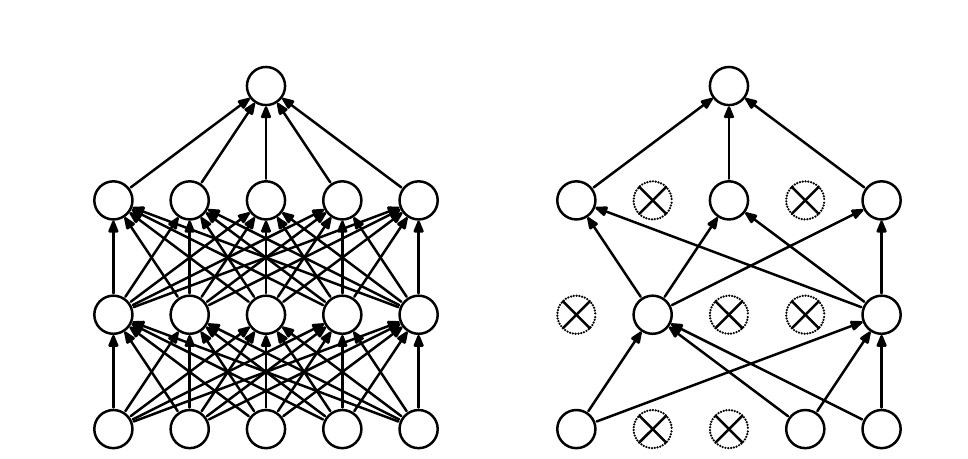
\includegraphics[width=\textwidth, keepaspectratio]{images/dropout.png}
	\centering 
	\caption{Ένα νευρωνικό δίκτυο με \en{dropout} (δεξιά) και χωρίς (αριστερά).}
	\label{fig:dropout}
\end{figure}

Η χρήση της τεχνικής \en{dropout} αναλογεί στη χρήση διαφόρων <<\tg{αραιωμένων}>> δικτύων που βασίζονται στο αρχικό.
Το αραιωμένο δίκτυο αποτελείται από τα στοιχεία που <<\tg{επέζησαν}>> της χρήσης \en{dropout} (βλ. \ref{fig:dropout}) και για κάθε παράδειγμα από το σετ εκπαίδευσης επιλέγεται τυχαία ένα αραιωμένο δίκτυο.
Έτσι, νευρωνικό δίκτυο με $n$ στοιχεία μπορεί να θεωρηθεί μια συλλογή από $2^n$ πιθανά αραιωμένα νευρωνικά δίκτυα τα οποία μοιράζονται βάρη με το αρχικό, και η εκπαίδευση του αρχικού ανάγεται στην εκπαίδευση της συλλογής αραιωμένων δικτύων. 
Για την εκτίμηση των επιδόσεων του συστήματος χρησιμοποιούμε όλα τα στοιχεία του νευρωνικού δικτύου, αλλά τα εξερχόμενα βάρη τους είναι πολλαπλασιασμένα με την αρχική πιθανότητα $p$ να κρατηθούν στη διαδικασία της εκπαίδευσης.